Following on from the design, this chapter discusses the process of taking the protocol from design to implementation on constrained devices. The chapter discusses the challenges faced throughout the implementation process, and the development on the event based operating system, Contiki, for the TelosB mote. 


\section{Implementation break-down} % (fold)
\label{sec:implementation_break_down}
In order to manage the implementation of the protocol, the development was broken down into functional components; these components were then implemented individually and tested, ensuring that the system functioned correctly before developing the next component.

Because of the functional similarities between the sensor and actuator, the initial development focused upon the communication model betweet the sensor and controller, with the sensor later modified to support the actuator functionality.

The implementation was broken down into the following:
\vspace{-5mm} 
\begin{enumerate}
	\item Test basic broadcast and unicast communication between two devices.
	\item Define packet structure, payload structures and device types.
	\item Implement broadcast device discovery and unicast response mechanism.
	\item Implement single channel device connections between devices after discovery.
	\item Implement sending sensor data and pings between connected devices.
	\item Implement multiple channel support for devices.
	\item Implement channel closing.
	\item Implement API bindings for application support.
	\item Implement mock applications on top of API.
\end{enumerate}
% subsection implementation_break_down (end)

% section software_engineering (end)

\section{Initial challenges} % (fold)
\label{sec:initial_challenges}
This section will discuss the challenges faced which initial choice of available hardware and software platforms.
\subsection{Arduino} % (fold)
\label{sec:arduino}
As described in the background chapter, \ref{sub:arduino}, the Arduino is unanimously the most popular open source constrained device available for consumers; thus developing an implementation of the protocol for it would allow it to be used with all the Arduino compatible devices currently available.

However, after much research into the platform, it was discovered that the Arduino did not natively support hardware interrupts from the available Ethernet network board.\cite{ArduinoEthernet} Instead any program expecting data from the network is forced to poll the Ethernet driver to check if any packets have arrived, resulting in a busy-wait. This busy-wait method of acquiring data from the network is extremely inefficient and directly opposite to what the protocol requirements and design aims to achieve, thus the Arduino was not chosen as the target development platform.
% section arduino (end)

\subsection{TelosB and operating system choice}
After deciding not to develop for the Arduino platform, the alternative platform available, due to the resources available in the School of Computing Science, was the TelosB mote. As described in section \ref{sub:telos_b_motes}, the TelosB mote is a widely used device within academia for research into wireless sensor networks and constrained operating systems. Because of this research, there are several operating systems to choose from when developing for the device, including TinyOS and Contiki.

Between TinyOS and Contiki there are some considerable differences, both in the programming model, event based vs hybrid (threaded \& event driven), and the structuring of the operating system, discussed previously in section \ref{sub:telos_b_motes}. Because of Contiki's programming model and language similarity to native C, it was chosen over TinyOS, in the hope that it would prove to be considerably easier to develop for.
% section initial_challenges (end)


\section{Telos B Mote and Contiki implementation} % (fold)
\label{sec:contiki}
After choosing to develop for the TelosB mote with Contiki, the next step involved getting to grips with how to best implement the system on the platform. This section discusses the process of implementing the system on the chosen platform, the various issues encountered, the overall structure dictated by the platform choice and the resulting system created. 

\subsection{Contiki \& Protothreads, a hybrid multi-threaded and event driven system} % (fold)
\label{sub:event_driven_system}
For implementing the system on Contiki, the hybrid programming model Contiki uses must first be understood. When developing an application in Contiki, the application can use one or more protothreads to run. Contiki's protothreads are lightweight, stackless threads which allow for linear code execution within an event-driven system, and also provide functionality to wait on events, either posted from other protothreads or from external events, such as a button press. This enables a developer to mix multiple threads of execution with an event-driven system to create a reactive system; this not only takes advantage of the constrained devices but also helps reduce the power consumption by sleeping when all threads are waiting on external events.
% subsection event_driven_system (end)

\subsection{Overall system architecture} % (fold)
\label{sub:protocol_system_architecture}
Before implementing the system, the overall architecture had to be decided upon, shown in figure \ref{fig:system_architecture}. In particular the method by which separate components, implemented as protothreads, interacted with each other within the system. For interaction two methods could be used:
\begin{itemize}
	\item Callback functions, by passing pointers of functions from the application to the API, when an event arrives such as a sensor reading, the appropriate function in the application can be called, passing it the related data. 
	\item Posting events, by defining new protocol specific events which the application program can wait on, and when an event occurs, such as a sensor reading arriving, the event is then rippled up to the application passing with it the related data.
\end{itemize}

For the majority of the system, the event based approach was chosen because fits in better with the event driven style of the rest of Contiki and also means the application can wait on events to occur and then wake up directly.
However, to simplify retrieving sensor readings and calling actions from the application, function pointers to functions which return the wanted data or carry out an action will be used, this enables the system to call the functions directly without having to wait for an event to be posted to the application and then waiting for one to return.
\begin{figure}[h!]
\centering
\includegraphics[scale=0.4]{implementation/img/system_architecture.1}
\caption{Overall system architecture}
\label{fig:system_architecture}
\end{figure}

% subsection protocol_system_architecture (end)

\subsection{Choosing the transport layer: uIP vs Rime} % (fold)
\label{sub:ip4_vs_ipv6_vs_rime}
Within the Contiki OS, several communication stacks are implemented, including a miniature IP stack called uIP (IPv4 \& IPv6) and the native Contiki Rime stack. Both stacks claimed to support the mechanisms required for the protocol, both broadcast and unicast, so either could be used. In an effort to enable easy integration into other IPv4 networks the uIPv4 stack was chosen. This meant that packets passed around the network could be routed to a gateway and sent to a neighbouring IPv4 network and possibly then on to the Internet without the need for translation. 
% subsection ip4_vs_ipv6_vs_rime (end)

\subsection{Problems Encountered} % (fold)
\label{sub:problems_encountered}
Whilst learning about and developing the system in Contiki, a variety of issues and problems occurred, each of which affected the time spent and complexity of the project in some way.
\subsubsection{Documentation} % (fold)
\label{ssub:documentation}
Whilst Contiki is a well developed and established operating system for constrained devices, such as the TelosB mote, the documentation for the OS and its libraries are mostly outdated, incomplete and provide no easy place to get started. Although most of the C syntax, structure and libraries remain consistent and intact, it's still fairly difficult to learn quite how the Contiki protothreads actually work and integrate with the system. Because of this a considerable amount of time was spent searching for up to date documentation.
% subsubsection documentation (end)

\subsubsection{Constrained resources} % (fold)
\label{ssub:constrained_resources}
Using the Contiki OS, which provides a significant amount of the standard C libraries that C programmers are familiar with, can provide some initial problems. An example of this is the inclusion of malloc, which in a normal x86 pc environment is very useful to enable run time allocation of data structures. But when used in a constrained environment where RAM is extremely limited, it becomes useless due to the limited heap space and the fragmentation of memory. 

Because of this, it is necessary to use static allocation to ensure memory is allocated correctly, but with this another problem arises. Because statically allocated memory is allocated at compile time, the size of the memory required needs to be known at compile time as well. When allocating fixed data structures this is not a problem, as the size of the data is already defined and known at compile time. Whereas, when allocating memory for the packets in the proposed protocol, it becomes difficult due to the varying payload lengths. In order to resolve this, the size to allocate for a packet can be defined as, size of the packet header + size of the largest payload. Doing this ensures that memory is always available for any packet, but at the same time for packets which don't have any payload the overallocation can waste a significant portion of the limited memory. In the implementation, this method of allocation is chosen, and each channel in the system is allocated one packet to send and receive messages.

As an alternative, which could save space at the cost of complexity, two pools of packets could be allocated; one pool stores packets with only the header, which would be used for sending messages with no command-specific payload, and the other pool stores packets with the maximum payload size, which would be used for all other command types. The complexity increases due to the need to ensure packets are allocated correctly between channels, ensuring that enough are available to service any incoming or outgoing request. In the case of resending packets, due to timeouts or repeat requests, if packets were returned to the pool after each use, the data for the retransmission would need to be regenerated; whereas in the implemented case, packets are only ever used by the channel to which they were assigned, so if the last packet needed to be resent, the data would still be contained within the stored packet, without the need of regeneration. 

% subsubsection constrained_resources (end)
\subsubsection{IPv4 Broadcast support} % (fold)
\label{sub:ipv4_broadcast_support}
After having chosen to use the uIPv4 UDP stack for communication, it was later discovered that the broadcast mechanism was just a stub.
The uIPv4 stack is implemented on top of the native Rime stack, so all IP packets are routed around using the Rime primitives for messages. Through much investigation it was found that when a broadcast packet is sent, it is given the normal ``all ones'' broadcast address, 255.255.255.255, but when the uIP layer is passed the packet to send, it detects the destination is outside of the local network and tries to find a gateway to send it over. Instead, the address should be recognised as a broadcast destination and then broadcast over the network.

After many attempts at contacting the Contiki developers community, no answer or solution was found; so instead a fix had to be created. As mentioned previously the uIPv4 stack is run over the Rime stack, and as discovered, using only a unicast Rime connection. In order to allow for broadcast packets to be sent, a new broadcast Rime connection needed to be created and correctly set up without breaking the existing code base. Once the broadcast code was in place, the system was tested to ensure it worked correctly and as expected for both unicast and broadcast packets.
% subsubsection ipv4_broadcast_support (end)

% subsection problems_encountered (end)

\subsection{Final implementation and API}
After deciding upon the architecture of the system, the communication stack to use and overcoming the various problems which arose throughout development, the implementation of the protocol on the TelosB motes with Contiki was completed. 

As shown in figure \ref{fig:protocol_architecture}, the implementation of the protocol uses only one protothread to receive, process and send any messages. The protothread is only active when an event occurs, either from the UDP stack, indicating a message has arrived, or from one of the timers in the system. In the implementation there are two types of timers, the clean up timer and the channel timer. The clean up timer is created once for the whole system and manages packet timeouts for reliable messages, occurring every 20ms. The channel timer, is instantiated once for each channel in the channel table; depending on the device, it either signals when the device should send out a sensor reading on a particular channel, which is defined when the channel is set up, or it defines when the actuator should send a ping to the connected controller to signify it is still alive. In the case of the controller it is used to signify by when it should receive a packet from a channel, defined as 3 times the predefined rate.

For communication between the protocol and the application, as discussed previously, events are used to pass information back to the application and commands are used to initiate actions, such as discovering devices, connecting to devices or closing connections.

Whilst the implementation adheres to the protocol design and specification proposed in chapter \ref{cha:design}, it does have some limitations in its current form. These include:
\begin{itemize}
 	\item Channel table limited to 10 channels due to memory constraints.
 	\item Two devices can create multiple channels between themselves. 
 \end{itemize} 



\subsection{Testing and Simulation} % (fold)
\label{sub:testing_and_simulation}
Throughout the implementation it was absolutely necessary to test the code as often as possible to ensure that it functioned correctly and as expected. Tests were performed both on real devices and within the provided simulator, Cooja, for the platform developed on, Contiki on TelosB motes. The Cooja simulator, shown in figure \ref{fig:simulator}, provided the ability to test scenarios which wouldn't be possible with the real devices, including testing with 10's of devices and with varying conditions such as radio strength and interference.

To test the implementation, unit tests were performed on each component of the system as it was developed, this was done to ensure that that each component functioned correctly before being integrated into the rest of the system. After which, the system was tested to see if the new component functioned correctly and did not break the existing code base. Using the Cooja simulator made it extremely easy to perform these tests and see how any changes effected the operation, without the need to reprogram each mote individually. 


\begin{figure}[h!]
\centering
\includegraphics[scale=0.5]{implementation/img/protocol_architecture.1}
\caption{Communication and threading architecture}
\label{fig:protocol_architecture}
\end{figure}

\begin{figure}[h!]
\centering
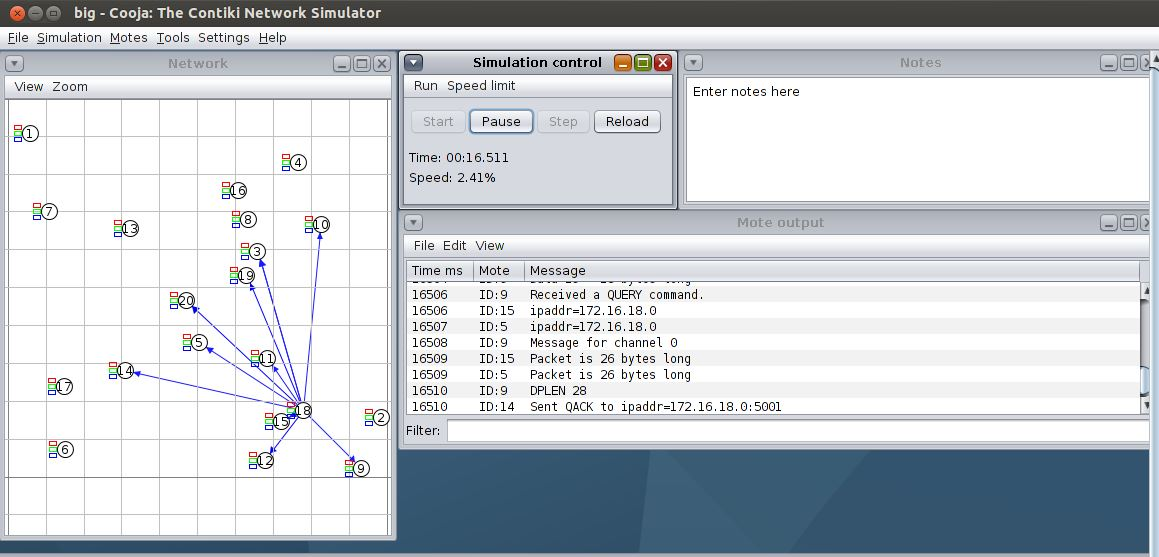
\includegraphics[scale=0.5]{implementation/img/cooja.jpg}
\caption{Cooja Simulator}
\label{fig:simulator}
\end{figure}

% subsection testing_and_simulation (end)


% section contiki (end)